\chapter{Realizações}\label{chp:realizacoes}

\section{Moverio BT-350}

% A \textit{Seiko Epson Corporation\texttrademark} introduziu o modelo no mercado com as vantagens de ser ajustável à cabeça; ser ideal para ser usado em lugares fechados ou ao ar livre; e possuir uma lente muito transparente, preparando-se para diversas modalidades de aplicações AR.

% \subsection{Especificações técnicas}

% \begin{description}
%     \item[\textbf{Tecnologia Óptica:}] \textit{Si-OLED (Silicon - Organic Light-Emitting Diode)  }
%     \item[\textbf{\textit{Field of View}:}] Aproximadamente 23°
%     \item[\textbf{Tela:}] 720p; 24-bit colour; 30 FPS
%     \item[\textbf{CPU e Memória:}]  Intel\textsuperscript{\textregistered} Atom\texttrademark x5, 1.44GHz Quad Core; 2GB RAM
%     \item[\textbf{Armazenamento:}] 16GB Armazenamento (32GB Expansível)
%     \item[\textbf{Conectividade:}] \textit{Wi-fi IEEE 802.11 (2G)}; \textit{USB 2.0}; \textit{Bluetooth BLE 4.0}
%     \item[\textbf{Sensores (\textit{Headset} e Controle):}] GPS; Giroscópio; e Acelerômetro
% \end{description}

% \begin{figure}
%     \centering
%     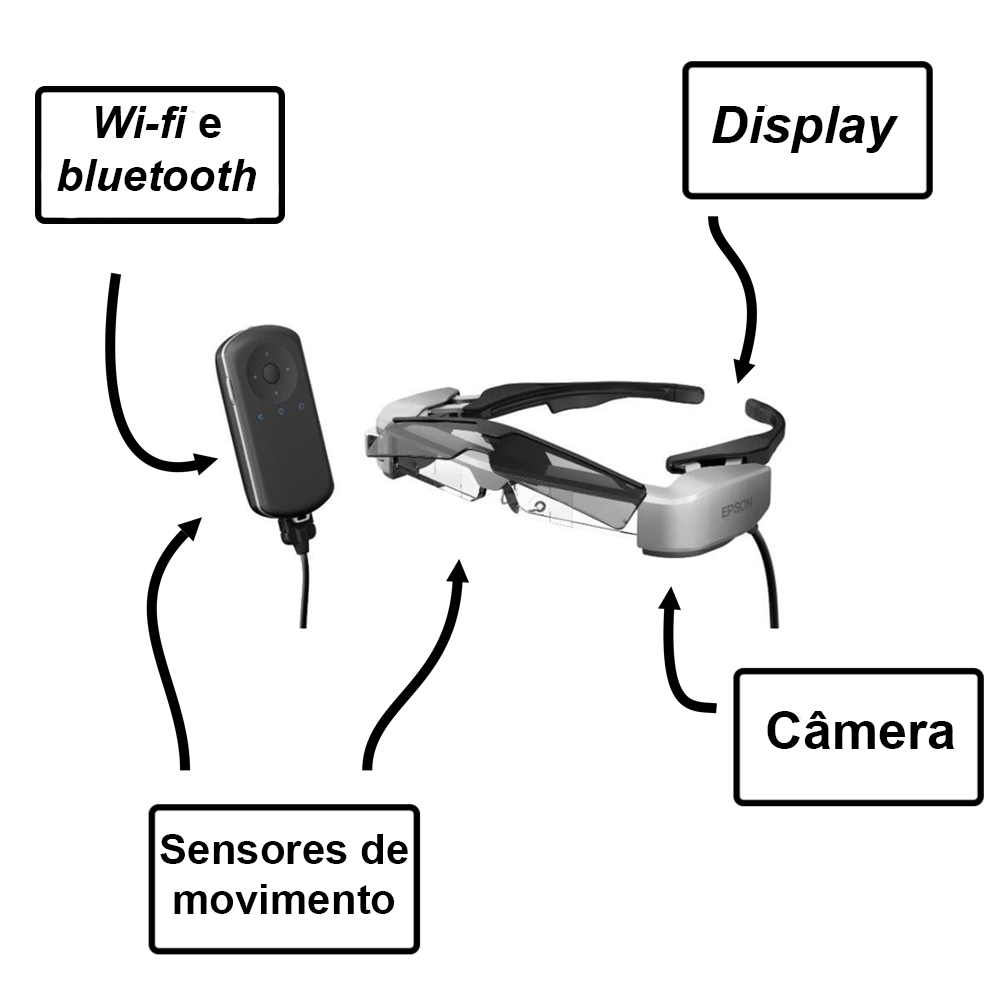
\includegraphics[width=.45\linewidth]{figuras/glass_comp.png}
%     \caption{Indicação da localização dos componentes nos óculos \textit{Moverio Bt-350}. Fonte: Autor.}
%     \label{fig:glass-parts}
% \end{figure}

\subsection{Documentação}

A \textit{Epson} disponibilizou uma documentação sobre as funcionalidades dos óculos e forneceu algumas ferramentas e aplicações exemplares para auxiliar os desenvolvedores de aplicativos do \textit{Moverio}. A tabela abaixo apresenta os arquivos da documentação e uma breve descrição:

\begin{center}
    \begin{tabular}{ |c|c| } 
        \hline
        \textbf{Arquivo} & \textit{\textbf{Descrição}} \\ 
        \hline
        \textit{CalibrationTool.apk} & Aplicativo de calibração da projeção da tela dos óculos\\ 
        \hline
        \multirow{2}{*}{\textit{CaptureTool.apk}} & Ferramenta que ajuda a capturar fotos para \\  & o mapeamento de novos marcadores e objetos \\
        \hline
        \multirow{2}{*}{\textit{TrainingToolWindows}} & Usa as imagens obtidas do \textit{CaptureTool.apk} e cria o \\ & \textit{dataset} para a detecção do novo marcador ou objeto  \\
        \hline
        \textit{Moverio\_AR} & Exemplo de cena que aplica funções do \textit{Moverio} no \textit{Unity} \\ 
        \hline
    \end{tabular}
\end{center}

Antes de prosseguirmos com os testes de cada programa, é importante denotar que o suporte da fabricante foi precário. No momento em que o projeto foi aprovado e acessou os \textit{sites} da fabricante, não foi encontrado a atualização de sistema, ficando com o \textit{Android 5.1} (\textit{API 22 Lollipop}) que estava muito desatualizado em relação ao mercado atual. Além disso, existia uma biblioteca exclusiva de aplicativos para o \textit{Moverio}, porém não para o \textit{BT-350}, mas para outros modelos com foco em usuário. A documentação existia, porém sua última atualização foi em julho de 2019, segundo os metadados dos arquivos. Por fim, infelizmente, o suporte do produto foi descontinuado enquanto a pesquisa utilizava sua documentação, ademais, os arquivos da documentação foram excluídos do \textit{site} da fabricante. O \textit{download} de todos os arquivos foi feito e reservado para os estudantes do laboratório.

\subsection{\textit{Calibration Tool}}

Segundo a fabricante, cada pessoa tem uma distância e um formato de rosto diferente, exigindo uma calibração específica para cada usuário \cite{Maruyama2018}. Essa calibração pode ser feita manualmente por meio da interface do \textit{CalibrationTool.apk}, que é instalado diretamente nos óculos. A calibração é efetuada ao ajustarmos uma imagem com o movimento da cabeça sobre o marcador da Figura \ref{fig:marker}. O processo é feito com cada olho, então fechamos o olho direito, ajustamos o esquerdo e fazemos o mesmo para o direito (Figura \ref{fig:calib}).

\begin{figure}[ht]
\centering
    \begin{subfigure}{0.45\textwidth}
        \centering
        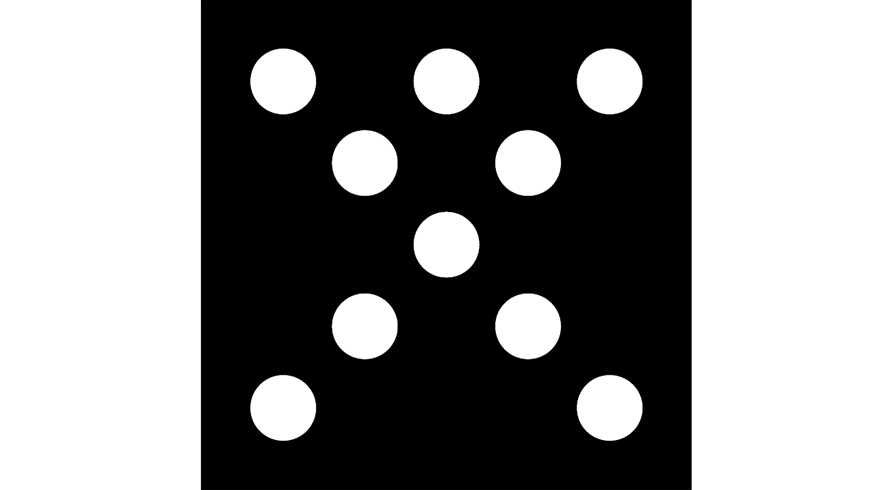
\includegraphics[width=.95\textwidth]{figuras/Marcador.png}
        \caption{Marcador da biblioteca \textit{Moverio}}
        \label{fig:marker}
    \end{subfigure}
    \begin{subfigure}{0.45\textwidth}
        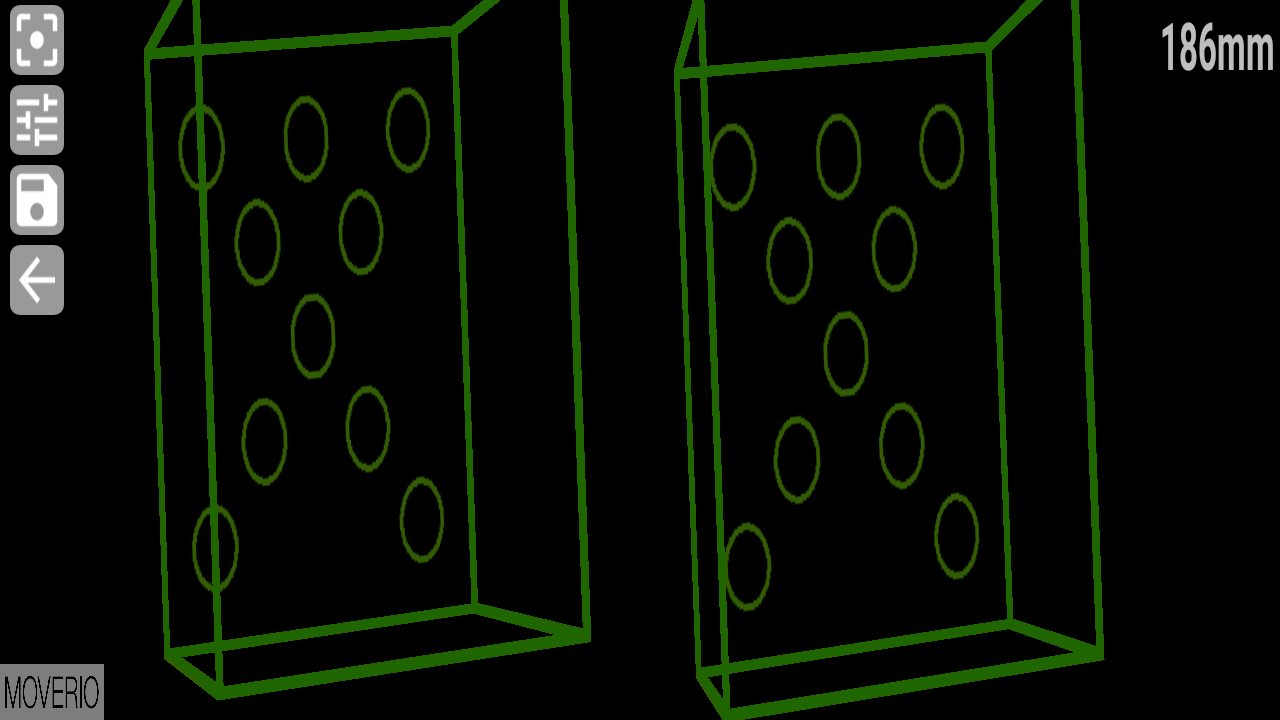
\includegraphics[width=.95\textwidth]{figuras/Calibration.png}
        \caption{Aplicativo fazendo a calibração}
        \label{fig:calib}
    \end{subfigure}
    \caption{Calibração usando marcador impresso e o aplicativo \textit{Calibration Tool} instalado nos óculos. Fonte: Autor.}      
    \label{fig:calibration}
\end{figure}

\subsection{\textit{Capture Tool}}

A \textit{Epson} forneceu um aplicativo para auxiliar a captura de fotos para o reconhecimento de novos objetos. O programa utiliza a imagem do marcador (Figura \ref{fig:marker}) que serve de referência de localização para a câmera que captura 16 imagens com a posição pré-definida. A obturação é automática quando o usuário entra na posição determinada, no entanto, a utilização do programa não é satisfatória na maioria das vezes: A câmera aciona automaticamente quando você está indo para a posição desejada, ou seja, ele obtura uma imagem embaçada pois sua cabeça ainda está em movimento.

\subsection{\textit{Training Tool}}

O \textit{software} tem o intuito de ampliar as possibilidades da detecção adicionando novos marcadores e objetos nos programas elaborados. Para treinarmos um  objeto precisamos importar o modelo 3D (\textit{STL}) no programa, e então utilizar as imagens coletadas do \textit{Capture Tool} para fazer um treinamento que habilitará a identificação do novo objeto. O primeiro teste foi realizado com uma lata de refrigerante, encontrado gratuitamente na \textit{internet}. Quando prosseguimos no programa, é pedido para escolhermos uma das imagem da captura e correlacionar pontos no objeto real da imagem e o modelo virtual (Figura \ref{fig:train-pt}). Após esse processo manual, o programa realiza a sobreposição do modelo no resto das imagens e libera uma ação de ajuste finais.

\begin{figure}[ht]
    \centering
    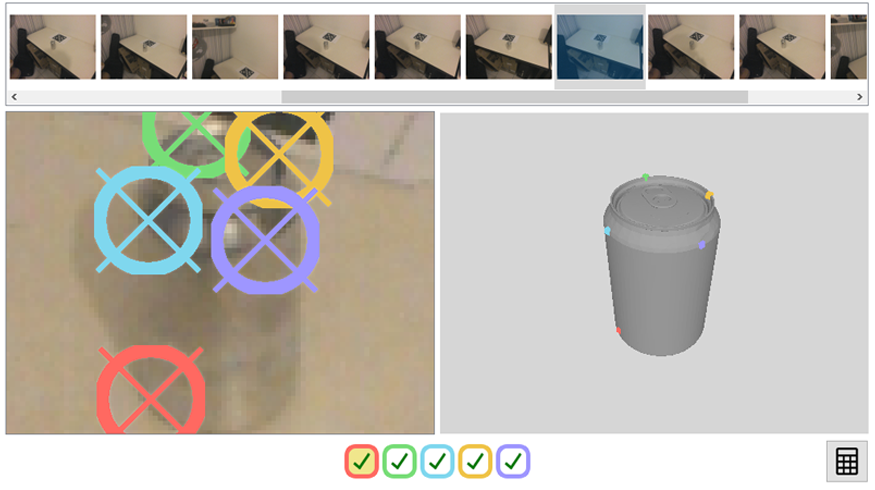
\includegraphics[width=.6\linewidth]{figuras/TrainingPoints.png}
    \caption{Tela da seleção de pontos. Fonte: Autor.}
    \label{fig:train-pt}
\end{figure}

O ajuste manual funciona muito bem, seu resultado é a figura \ref{fig:ajuste-manual}. O próximo passo é esperar o programa encontrar a posição automaticamente no resto das imagens, porém, isso não ocorre como o desejado. A Figura \ref{fig:estimation} representa uma falha na estimação de posição da lata, normalmente, pensaríamos em descartar essa imagem da lista, no entanto, essa é a melhor tentativa que o programa fez, os demais erram tanto que a latinha mal aparece na imagem. Ao tentar realizar um reajuste nessa imagem, o programa impede a ação e notifica que a diferença é muito grande em relação ao primeiro ajuste, o que impossibilita o resultado de ser satisfatório.

\begin{figure}[ht]
\centering
    \begin{subfigure}{0.45\textwidth}
        \centering
        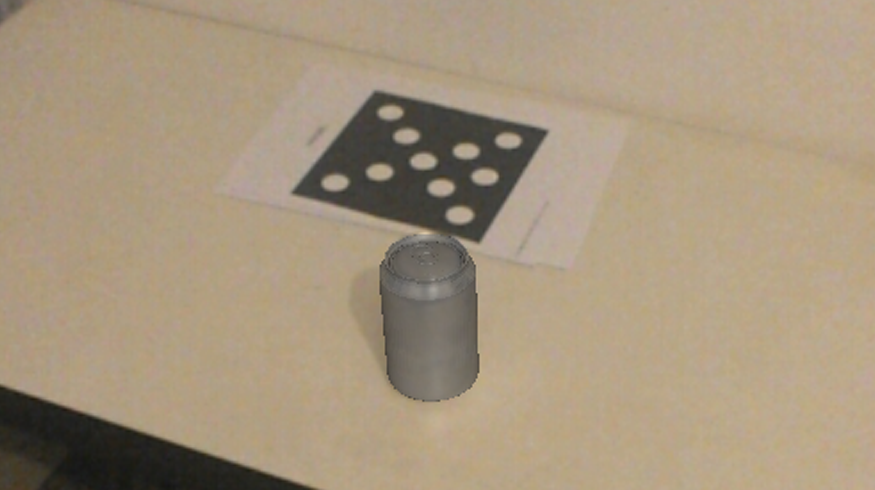
\includegraphics[width=.95\textwidth]{figuras/Latinha-ideal.png}
        \caption{Ajuste manual da Figura \ref{fig:train-pt}}
        \label{fig:ajuste-manual}
    \end{subfigure}
    \begin{subfigure}{0.45\textwidth}
        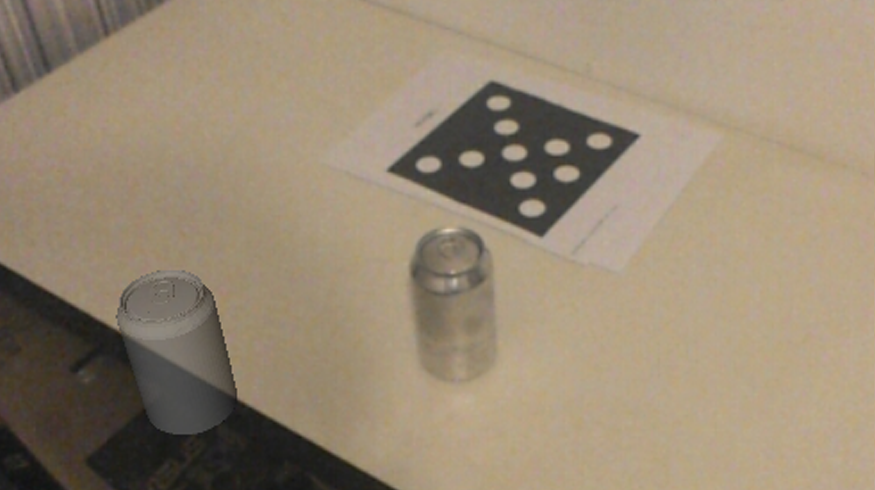
\includegraphics[width=.95\linewidth]{figuras/Latinha-errada.png}
        \caption{Posição encontrada pelo programa }
        \label{fig:estimation}
    \end{subfigure}
    \caption{Tentativa do treinamento na detecção da lata de refrigerante. Fonte: Autor.}
    \label{fig:pose-estimation}
\end{figure}

% As primeiras suspeitas disso ocorrer foi a mensagem inicial que o programa alertou que o modelo possui muitos detalhes, então tentamos criar nosso próprio modelo simplificado com uma forma menos simétrica que a lata. Um papel sulfite foi dobrado em formato de cone não regular e modelado no computador como pode ser visto na Figura \ref{fig:ConeAR}.

% \begin{figure}[ht]
% \centering
%     \begin{subfigure}{0.45\textwidth}
%         \centering
%         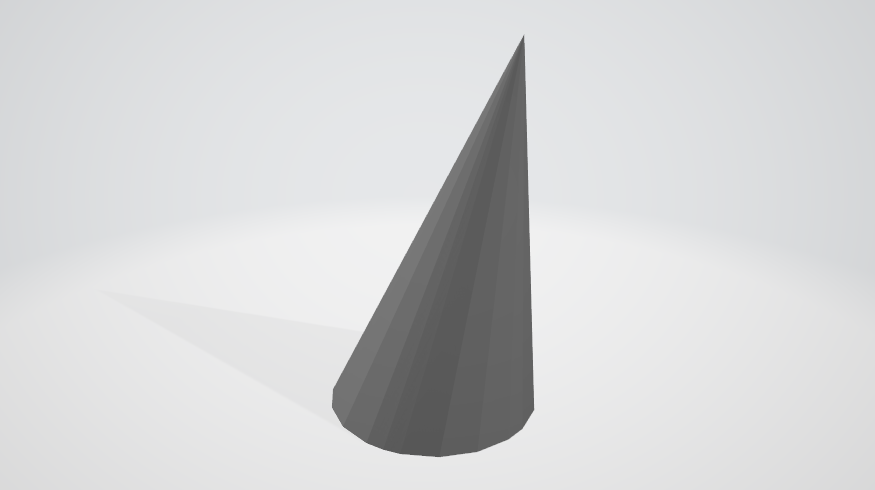
\includegraphics[width=.95\textwidth]{figuras/ConeSTL.png}
%         \caption{Modelo em \textit{STL} do objeto}
%         \label{fig:cone-stl}
%     \end{subfigure}
%     \begin{subfigure}{0.45\textwidth}
%         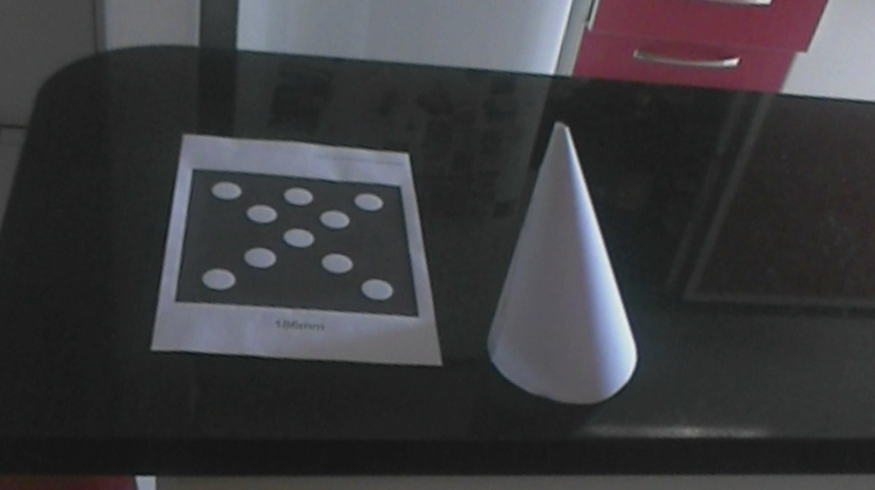
\includegraphics[width=.95\linewidth]{figuras/Cone.png}
%         \caption{Sessão de captura feita em uma mesa preta}
%         \label{fig:cone-training}
%     \end{subfigure}
%     \caption{A tentativa com o cone foi feita em outro ambiente com o fim dar um maior destaque no objeto. Fonte: Autor.}
%     \label{fig:ConeAR}
% \end{figure}

% O resultado foi muito semelhante ao erro encontrado na tentativa da lata, o programa é incapaz de predizer a posição do objeto para as demais imagens como acontece na Figura \ref{fig:pose-estimation}. O erro pode ter ocorrido da variação da iluminação, na lata ou da mesa ter reflexos do ambiente, ou mesmo que ambos os objetos não possuem textura.

\subsection{\textit{Moverio AR}}\label{chp:moverio-unity}

\textit{Unity} é um programa voltado para o desenvolvimento de jogos em múltiplas plataformas, sendo o \textit{Android} uma delas, e com o apoio da USP, temos acesso a mais recursos para os projetos desenvolvidos nele \cite{UnityOficial}. A documentação da forneceu um programa de exemplo para \textit{Unity} que pode reconhecer um carrinho de papel e sobrepor com animações em AR. Para o teste, supomos que ele funcionaria com uma imagem no computador, pois ele não pode diferenciar tridimensionais e bidimensionais pela limitação da câmera. De fato, isso ocorreu e o teste foi registrado na figura \ref{fig:papercar-tests}.

\begin{figure}[ht]
    \centering
        \begin{subfigure}{.45\textwidth}
            \centering
            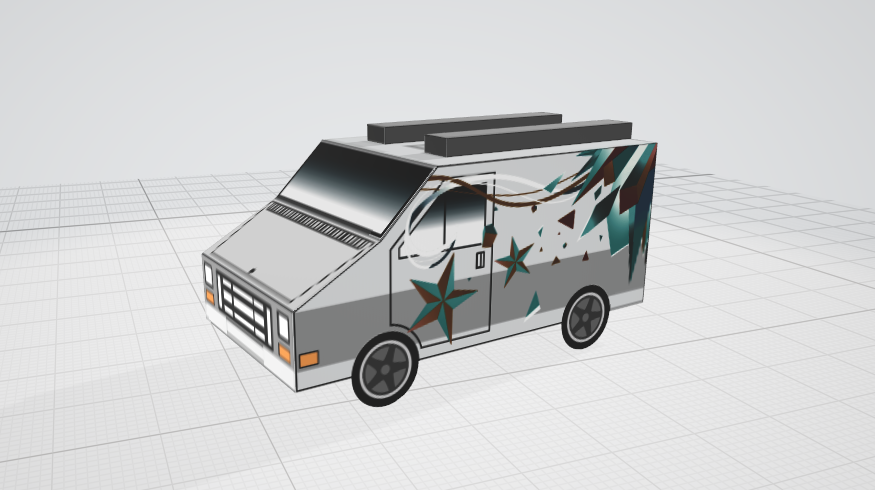
\includegraphics[width=.95\textwidth]{figuras/PaperCar.png}
            \caption{Modelo virtual do carrinho de papel}
            \label{fig:papercar-stl}
        \end{subfigure}
        \begin{subfigure}{.45\textwidth}
            \centering
            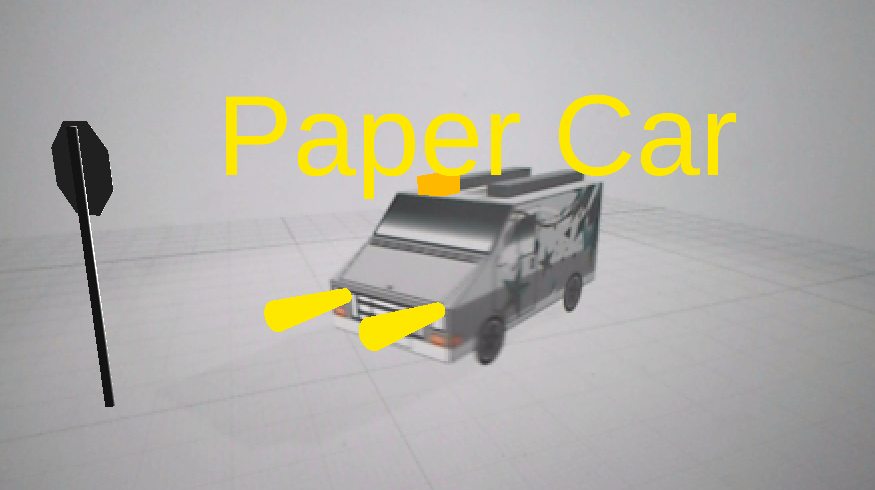
\includegraphics[width=.95\textwidth]{figuras/PaperCarAR.png}
            \caption{Sobreposição em AR com \textit{Moverio}}
            \label{fig:papercar-ar}
        \end{subfigure}
        \caption{Resultados adquiridos dos testes da documentação \textit{Moverio} no \textit{Unity}. Fonte: Autor.}
        \label{fig:papercar-tests}
\end{figure}

\section{Estudos em desenvolvimento Android Studio}

O desenvolvimento de aplicativos para \textit{Android} foi estudado nos primeiros meses da pesquisa. Nessa parte do projeto, a pesquisa teve um aspecto mais técnico, que foi necessário para a programação das futuras aplicações que estariam por vir. A \textit{IDE} (ambiente de desenvolvimento integrado) utilizada foi o \textit{Android Studio}, que foi sugerida pelo curso adquirido da \textit{Udemy} \cite{udemy}.

Após as primeiras semanas de aprendizado \textit{Android}, foi iniciado uma pesquisa sobre o desenvolvimento de aplicativos voltados a realidade aumentada. Porém, antes de irmos diretamente nisso, um interessante teste foi realizado com \textit{OpenCV},  que consistiu em realizar a primeira manipulação das imagens da câmera \cite{opencv}. A experiência foi proveitosa para o aprendizado da integração de ferramentas externas ao projeto padrão da plataforma e que, ademais, será feito muitas vezes até a conclusão da pesquisa.

A primeira biblioteca de realidade aumentada a ser testada foi o \textit{Google Sceneform} \cite{Sceneform}. Muitos problemas foram encontrados na integração dos \textit{plugins} com o \textit{Android Studio}, pois este precisava estar em uma versão antiga específica para funcionar. Após a instalação, foi possível ver a primeira projeção em realidade aumentada em um simulador de \textit{smartphone} no computador (figura \ref{fig:sceneform-sim}). Restava testar o aplicativo para um \textit{smartphone} real, porém o afastamento dos integrantes do laboratório pela pandemia, e a falta de dispositivos compatíveis à minha disposição, causaram um atraso nos testes. Felizmente, foi gerado um arquivo que permite a instalação à distância e o aplicativo funcionou com sucesso nos celulares da equipe (figura \ref{fig:sceneform-real}).

\begin{figure}[ht]
\centering
    \begin{subfigure}{.45\textwidth}
        \centering
        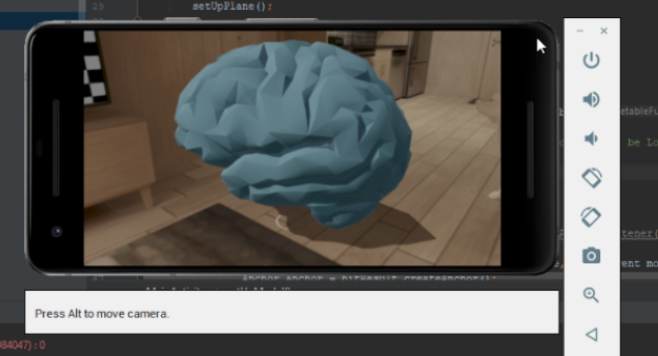
\includegraphics[width=.95\textwidth]{figuras/sceneform.png}
        \caption{Simulação da projeção AR }
        \label{fig:sceneform-sim}
    \end{subfigure}
    \begin{subfigure}{.45\textwidth}
        \centering
        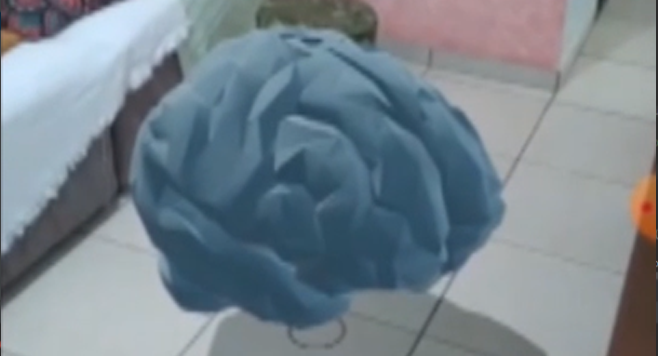
\includegraphics[width=.95\textwidth]{figuras/sceneformAR.png}
        \caption{Teste do aplicativo com \textit{Smartphone} real}
        \label{fig:sceneform-real}
    \end{subfigure}
    \caption{Resultados adquiridos com o \textit{Google Sceneform}. Fonte: Autor.}
    \label{fig:sceneform-tests}
\end{figure}

Prosseguindo os estudos de aplicativos AR, percebemos que os problemas de versão tidos com o \textit{Sceneform} estavam sendo reparados pelo \textit{Google} e adaptados em um novo programa: \textit{Google ARCore Services} \cite{arcore-googleplay}. Sua proposta é que uma biblioteca seja instalada no celular para que os aplicativos tenham acesso, trazendo a vantagem da redução do tamanho das aplicações produzidas. No entanto, somente uma lista restrita de \textit{smartphones} modernos podem instalar essa biblioteca, a justificativa dos desenvolvedores é a compatibilidade com o sistema \cite{arcore-list}.

Seguido disso, durante a pesquisa foi encontrado uma nova ideia \textit{open-source}, também do \textit{Google}, chamado \textit{Mediapipe}, que tinha a proposta de entregar muitas ferramentas de visão computacional com ML (\textit{machine learning}) integrado \cite{mediapipe-docs}. O projeto foi iniciado em julho de 2019, e tem ganhado mais popularidade por ser gratuito, multi-plataforma e facilitar muito a aplicação de ML para \textit{Android}, \textit{iOS}, e PC. No momento da descoberta, não era conhecido a compatibilidade do \textit{Mediapipe} com \textit{API} antigas de \textit{Android} e muito menos o seu comportamento em óculos de realidade aumentada, por isso, a ideia foi reservada.

% LISTA RESUMIDA ANDROID STUDIO
% \begin{description}
%    \item Um sumário das opções testadas com breves comentários abaixo:
%    \item[\textit{Google Sceneform}] É um \textit{plugin} para \textit{Android Studio} que introduz muitas ferramentas para o desenvolvimento de aplicativos AR. Funciona somente em \textit{Android} com a \textit{API} 24 ou superior. Seu projeto foi arquivado em meados de 2020. 
%    \item[\textit{Google ARCore Services}] Pode se considerar o sucessor das ideias do \textit{Sceneform}. Ele fornece uma biblioteca de ferramentas sofisticadas para AR e atualizações frequentes. Funciona somente em uma lista estrita de \textit{smartphones} modernos. 
%    \item[\textit{Mediapipe}] Fornece uma grande quantidade de ferramentas baseadas em \textit{Machine Learning} para visão computacional. Projeto iniciado em junho de 2019 e ganhando mais força recentemente. Pela recente criação, não é conhecido seu comportamento em \textit{API} antigas (28 ou anterior).
% \end{description}

% \begin{figure}[ht]
% \centering
%     \begin{subfigure}{0.45\textwidth}
%         \centering
%         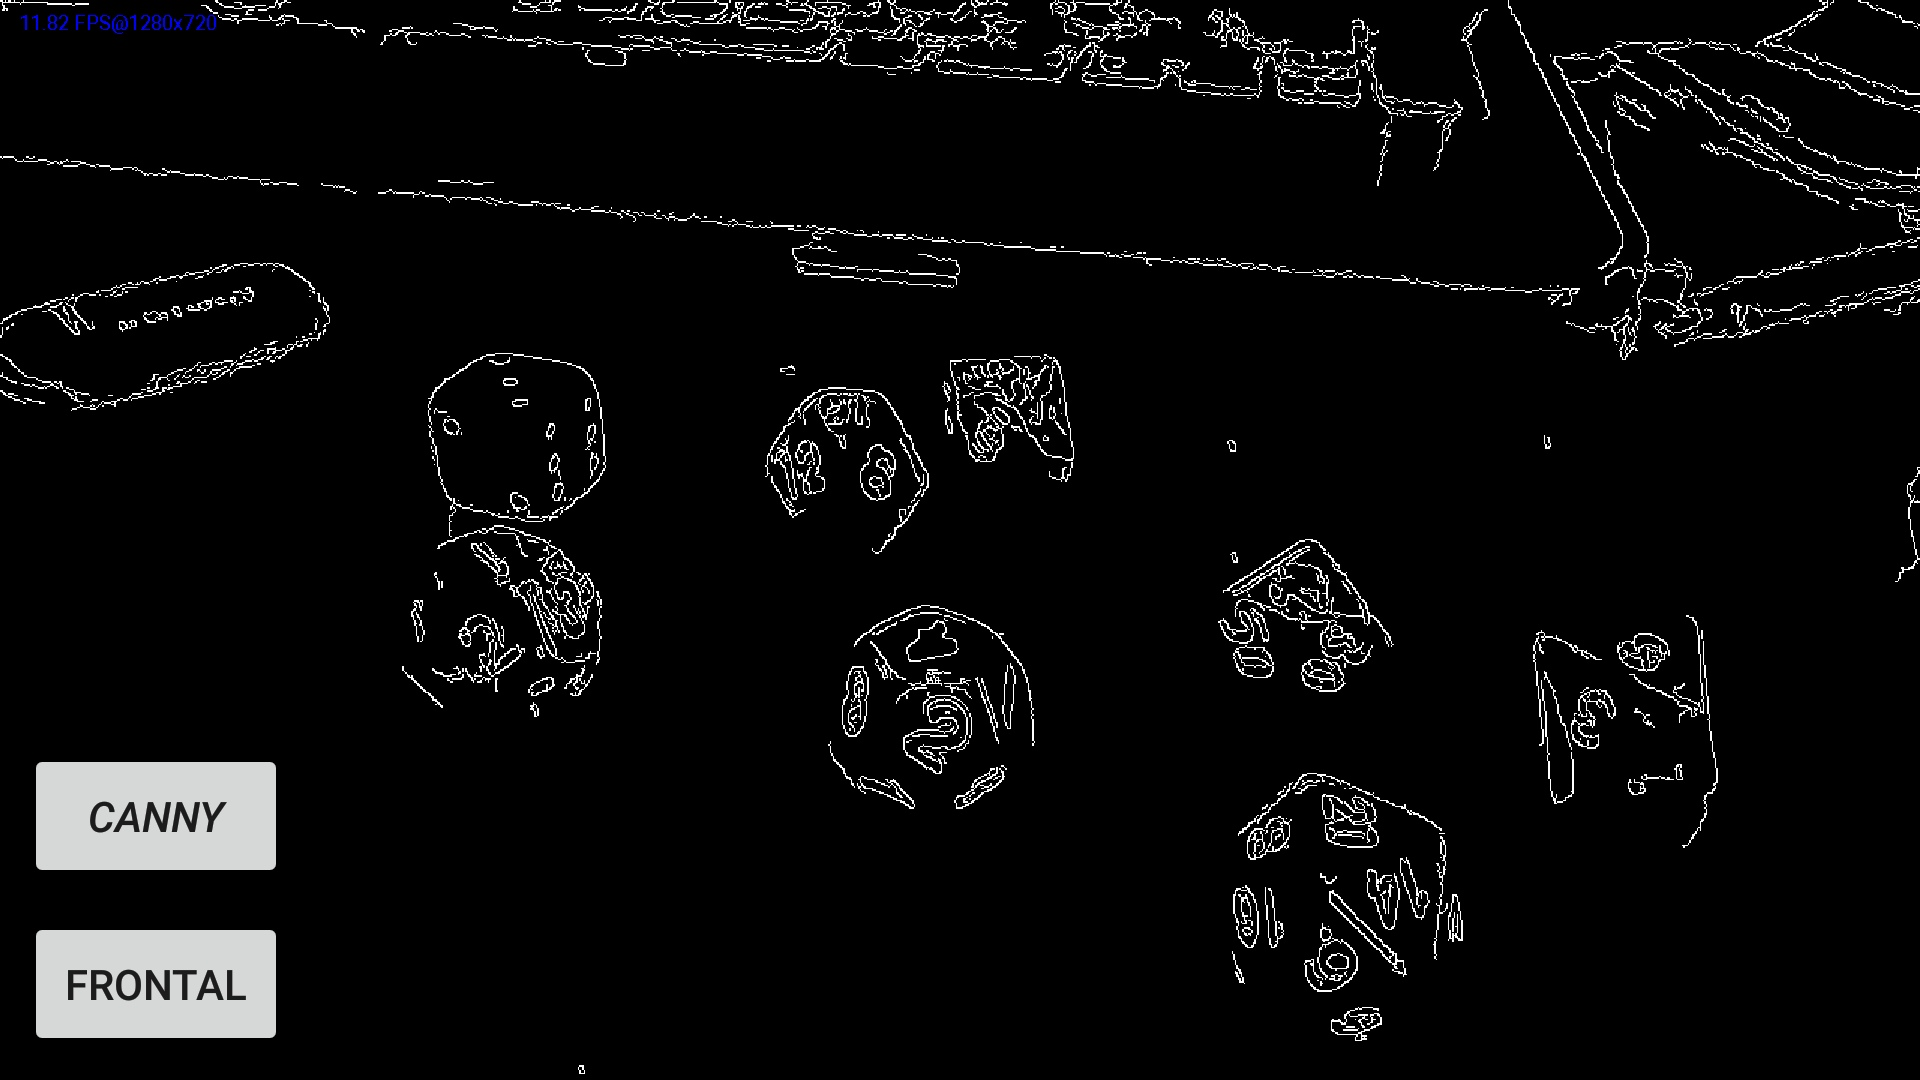
\includegraphics[width=.95\textwidth]{figuras/opencv-canny.jpg}
%         \caption{Aplicativo com \textit{OpenCV} integrado no \textit{Android}}
%         \label{fig:canny}
%     \end{subfigure}
%     \begin{subfigure}{0.45\textwidth}
%         \centering
%         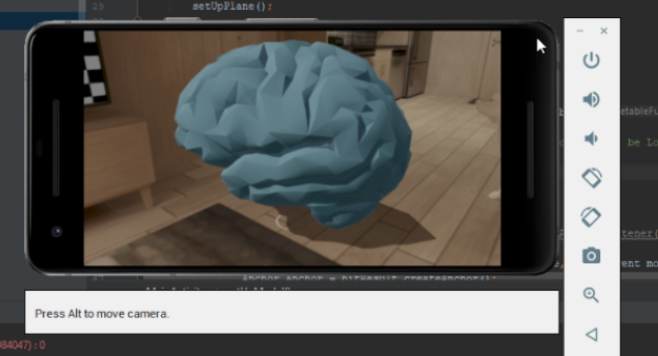
\includegraphics[width=.95\textwidth]{figuras/sceneform.png}
%         \caption{Primeiro aplicativo AR para \textit{Android}}
%         \label{fig:sceneform}
%     \end{subfigure}
%     \begin{subfigure}{0.45\textwidth}
%         \centering
%         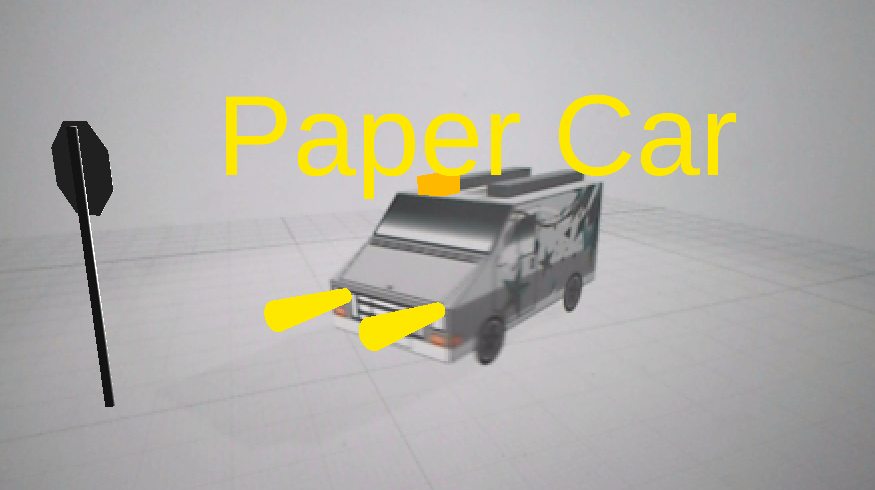
\includegraphics[width=.95\textwidth]{figuras/PaperCarAR.png}
%         \caption{Aplicativo de exemplo fornecido pela \textit{Epson}}
%         \label{fig:papercarr}
%     \end{subfigure}
%     \begin{subfigure}{0.45\textwidth}
%         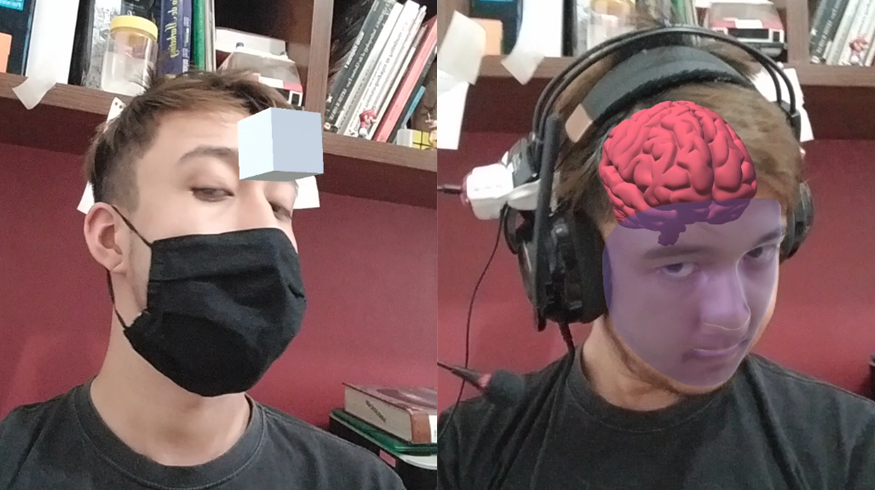
\includegraphics[width=.95\linewidth]{figuras/VCranium.png}
%         \caption{Primeira versão do \textit{VCranium}}
%         \label{fig:vcranium_alpha}
%     \end{subfigure}
%     \caption{Histórico de realizações da pesquisa até a primeira entrega parcial. Fonte: Autor.}
%     \label{fig:historico}
% \end{figure}

O que podemos concluir do desenvolvimento de aplicações em realidade aumentada com \textit{Android Studio} é que mesmo existindo ferramentas robustas de criação de \textit{apps} em AR, eles são restritos às novas versões de \textit{Android}, que por sua vez, estão presentes somente em dispositivos de nova geração, i.e, de lançamento posteriores a 2018. Por fim, a incompatibilidade das bibliotecas com o sistema e a construção dos óculos AR foram os motivos para a procura de um novo ambiente de desenvolvimento, que seja mais versátil e comporte bem com os recursos do \textit{Moverio BT-350}.

\section{Estudos de desenvolvimento Unity}

O programa apresentado no capítulo "\nameref{chp:moverio-unity}" foi o único programa em \textit{Unity} disponibilizado na documentação dos óculos, o projeto foi elaborado no \textit{Unity} 2017, mesmo com alguns alertas de incompatibilidade, o projeto pôde ser compilado com êxito e funcionou nos óculos. Novamente, a falta do suporte da \textit{EPSON} deixou incerto se era uma boa opção construir um aplicativo somente baseado na documentação disponível. Por isso, iniciamos novamente uma pesquisa sobre as ferramentas para suporte de AR nessa plataforma.

O \textit{Vuforia} foi o primeiro \textit{plugin} a ser testado no ambiente do \textit{Unity} \cite{Vuforia}. Atualmente, ele apresenta mais opções rastreio para AR, mas no momento em que foi experimentado pela pesquisa as opções eram de usar imagens e algumas formas 3D como marcadores para suas projeções. Foi testado a detecção de imagem com um pedaço da logo da \textit{Coca-cola\texttrademark} como alvo, a figura \ref{fig:vuforia-tests} ilustra os resultados.

\begin{figure}[ht]
    \centering
    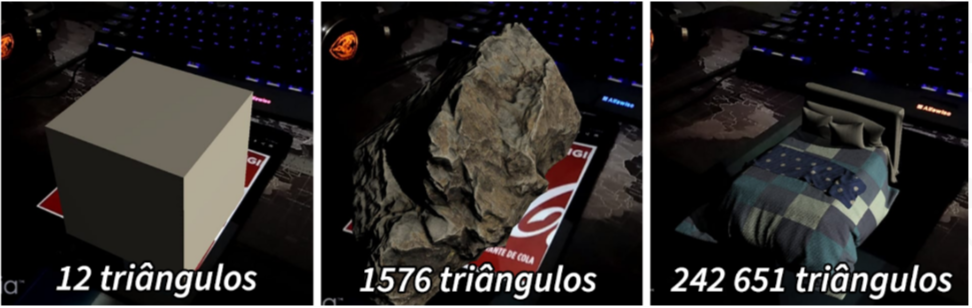
\includegraphics[width=.85\linewidth]{figuras/Vuforia.png}
    \caption{Testes com diferentes modelos de diferentes complexidades, constatando performance acima de 15 quadros por segundo em todos os casos. Fonte: Autor.}
    \label{fig:vuforia-tests}
\end{figure}

As formas de detecção tridimensionais não eram compatíveis com a detecção da posição da cabeça de um paciente, por isso esse recurso não foi testado. O \textit{Vuforia} é uma ferramenta que trabalha com \textit{Android} de \textit{API} 23 ou superior, infelizmente, também incompatível com o \textit{Moverio BT-350} que possui uma \textit{API} 22 e sem chances de atualização. Outras ferramentas foram encontradas como o \textit{Wikitude\texttrademark} que também era para \textit{API} 23 \cite{wikitudes}, porém uma outra ferramenta denominada \textit{ARFoundation} que estima a posição da face humana chamou a atenção por termos a oportunidade de criar uma demonstração da ideia final do projeto nos óculos \cite{arfoundation-docs}.

\begin{figure}[ht]
    \centering
    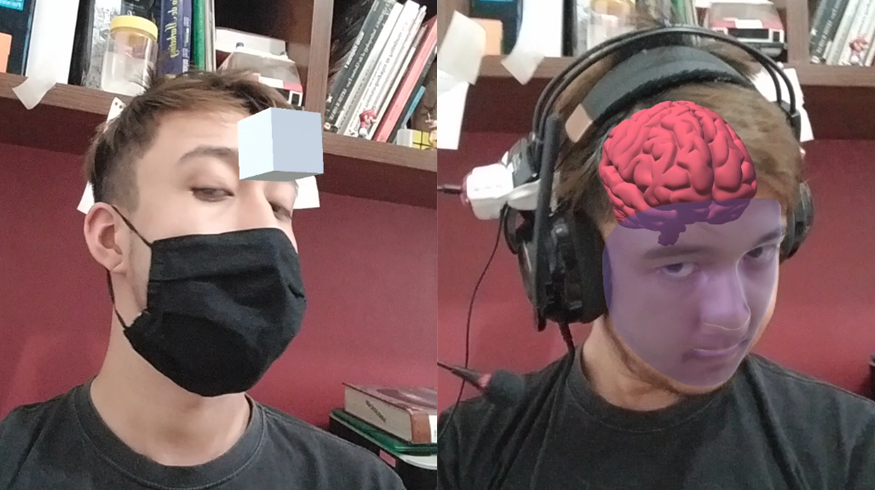
\includegraphics[width=.6\linewidth]{figuras/VCranium.png}
    \caption{A primeira imagem foi o primeiro teste com a projeção de um cubo na região da testa. A segunda detalha a superfície estimada da face e a projeção do cérebro. Fonte: Autor.}
    \label{fig:arfoundation}
\end{figure}

A instalação do \textit{ARFoundation} foi feita no \textit{Unity 2018} e apresentou compatibilidade com celulares de \textit{API 28} ou superior. Os testes consistiram em utilizar a posição da face encontrada pelo \textit{plugin} para projetar um objeto em referência desses dados. A aplicação teve um ótimo resultado e foi possível apresentar o objetivo principal para professores e médicos da área pela aproximação visual dos testes com o resultado final esperado, visto na figura \ref{fig:arfoundation}. Nesse momento, criamos um nome fantasia para facilitar as apresentações do projeto: \textit{VCranium}.

Retornando ao objetivo prático de encontrar um meio de desenvolver o projeto, concluímos que temos muitas opções disponíveis de desenvolvimento, mas sem muito suporte para o \textit{Moverio BT-350}. O \textit{Unity} foi escolhido para seguir a pesquisa pela sua facilidade de elaboração de cenários tridimensionais e compatibilidade com o sistema de outros óculos de AR do mercado. Dessa maneira, podemos garantir que os próximos trabalhos que serão desenvolvidos, não dependem do equipamento que temos hoje, i.e, se futuramente precisarmos trocar para um óculos mais moderno, uma adaptação será feita e aproveitaremos o material produzido até o momento.

Dado o histórico de testes do projeto, foi decidido prosseguir sem depender de \textit{plugins} e bibliotecas \textit{closed-source}, isso garantirá um maior controle do \textit{software} elaborado e também exigirá um estudo mais aprofundado de como os algoritmos de visão computacional funcionam. Essa mudança trará um contato maior com problemas discretizados de programação, auxiliando o processo do estudo e apresentação de dúvidas em seminário para os estudantes e professores dessa área de pesquisa na universidade.

\section{Revisão bibliográfica}

Aqui podemos analisar com mais atenção os artigos da literatura e suas diferentes soluções para sistemas de realidade aumentada aplicados em cirurgias. O trabalho que mais auxiliou a pesquisa foi uma revisão literária de aplicações em AR para neurocirurgias: \textit{"Enhancing Reality: A Systematic Review of Augmented Reality in Neuronavigation and Education"} \cite{enhancedvision}. Esse artigo faz uma breve apresentação da aplicabilidade de AR em ambiente cirúrgico e tabela as informações de doze pesquisas mostrando as patologias tratadas; descrição de método; e resultado da precisão da projeção em AR.

Dentre as pesquisas descritas estava o artigo de Maruyama: \textit{Smart Glasses for Neurosurgical Navigation by Augmented Reality} \cite{Maruyama2018}. Sua equipe de pesquisadores construíram um sistema que utilizava os óculos \textit{Moverio BT-200}, um modelo que se assemelha muito com o que possuímos no laboratório, para auxiliar a visualização de tumores cerebrais em dois pacientes, além disso, foi também possível exibir a escalpe; o crânio; e os vasos da superfície do cérebro nos óculos.

\begin{figure}[ht]
    \centering
    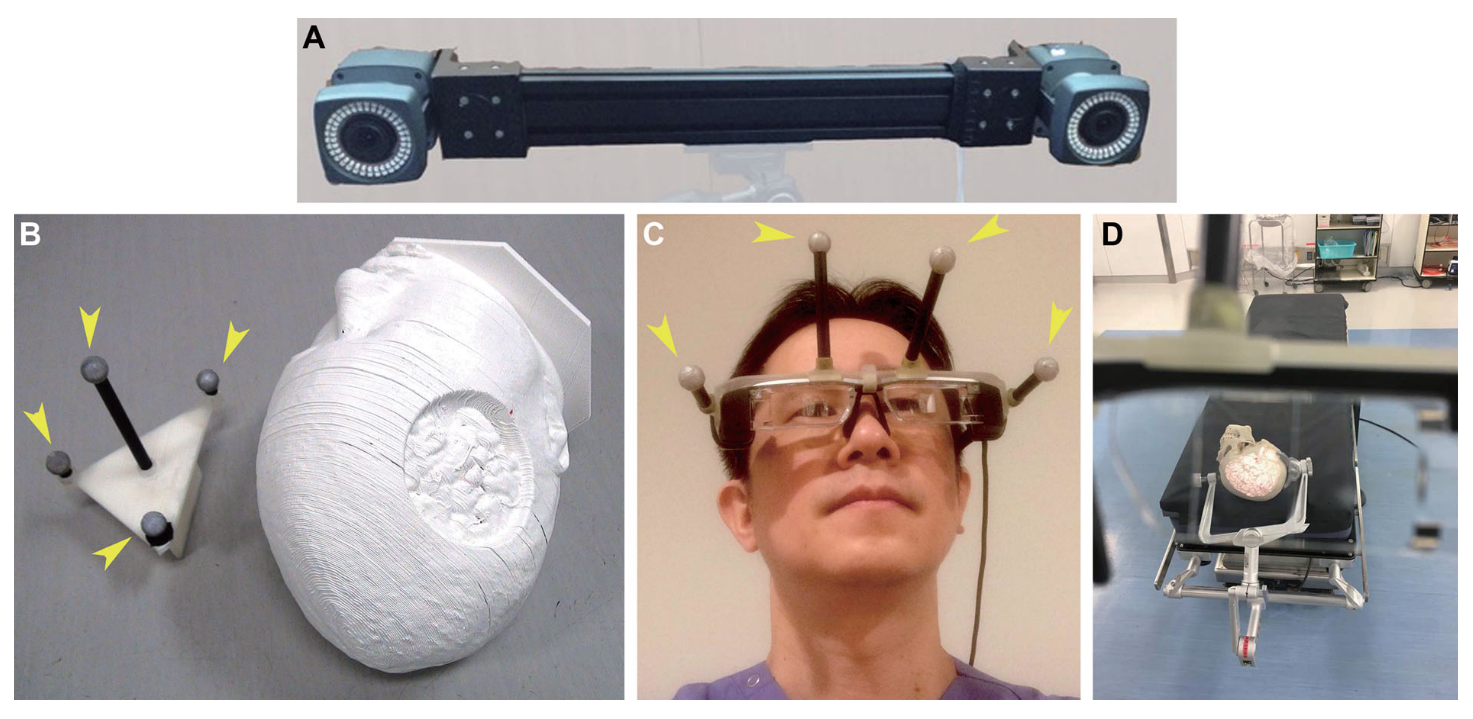
\includegraphics[width=.65\linewidth]{figuras/Maruyama.png}
    \caption{(A) Duas câmeras para detectar movimento, (B) Marcadores para paciente, (C) Marcadores nos óculos, (D) Visualização nos óculos. Fonte: \cite{Maruyama2018}.}
    \label{fig:maruyama}
\end{figure}

\begin{figure}
    \centering
    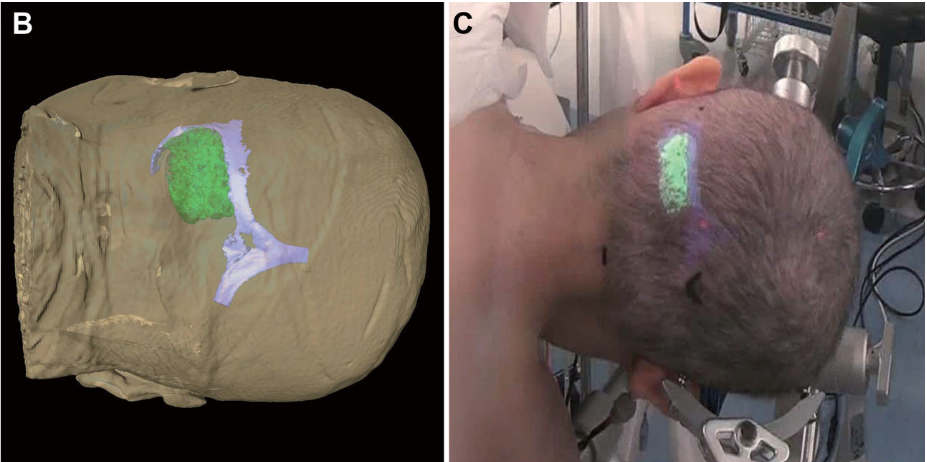
\includegraphics[width=.65\linewidth]{figuras/maruyama-overlay.png}
    \caption{(B) Computação gráfica da reconstrução do cérebro do paciente, (C) Visualização em AR antes da incisão. Fonte: \cite{Maruyama2018}.}
    \label{fig:maruyama-overlay}
\end{figure}

O método que o artigo utilizou apresentou a dinâmica da integração de componentes para uma arquitetura de um sistema AR: Empregar câmeras estereoscópicas para a detecção de marcadores nos óculos e na cabeça do paciente; relacionar com os dados da reconstrução 3D do cérebro; utilizar parâmetros da calibração; e fazer a exibição nos óculos. Por meio desse sistema, o resultado obtido é visto na figura \ref{fig:maruyama-overlay}.

A precisão da projeção, segundo o artigo, foi de \(2.1 \pm  1.3\,mm\) com a mediana de \(1.8\) e a remoção total de \(5\) tumores com sucesso e sem complicações pós-operatórias. Além disso, o sistema tem uma interface de fácil utilização e conveniência para o médico, sendo possível desabilitar a projeção em qualquer momento da cirurgia, teve um custo menor que os sistemas de neuronavegação convencionais e, por fim, pode ser instalado em outros óculos de AR comerciais disponíveis, portanto, não se limitando ao seu modelo do \textit{Moverio} \cite{Maruyama2018}.

Os resultados apresentados por essa pesquisa e que a conjectura apresentada na seção anterior - aplicação baseado no \textit{Unity} para a compatibilidade com mais óculos do mercado - foram confirmados possíveis. Contudo, antes de simplesmente seguir os passos de Maruyama, decidimos fazer uma listagem das arquiteturas utilizadas em outros sistemas para tentar ponderar suas características para optarmos pela opção que mais atende as necessidades da pesquisa.

\section{Elaboração do VCranium}\label{chp:criacao-vcranium} 

\subsection{Arquitetura do Sistema}

A definição da arquitetura do sistema é muito importante para configurar o funcionamento do sistema, estabelecer suas vantagens e desvantagens, e implicará como nós trabalhos em seu desenvolvimento. Para isso, a equipe realizou reuniões e debates para estabelecer uma solução que seja compatível para um período de seis meses e respeitando as medidas de prevenção por afastamento pela pandemia de COVID-19. Ainda assim, precisamos de uma arquitetura versátil e que objetiva facilitar a mudança de métodos de estimação a posição da projeção em AR. 

Para tal, dividiremos o sistema em computador e óculos: O computador estima a posição da projeção e os óculos fazem a visualização nos olhos do usuário. Isso simplifica a mudança de método aplicado pelo computador, melhorando a recepção de novos algoritmos da equipe de estudos do laboratório. Esse invento foi aplicado no artigo de Maruyama, que utilizou um \textit{software} de visualização médica e enviou os dados de exibição para o \textit{Unity} nos óculos \cite{Maruyama2018}. Com a definição dos componentes da arquitetura, deve ser definido uma comunicação entre os dispositivos. Um exemplo da literatura foi o uso do computador para adquirir informações de sinais vitais de equipamentos médicos e o envio para os óculos via \textit{TCP/IP} (Protocolo de Controle de Transmissão / Protocolo de \textit{Internet}) \cite{Arpaia2021}.

Utilizando o recurso de conexão \textit{wireless} dos óculos, podemos nos conectar com o computador via \textit{LAN} (Rede de área local). Na questão da oscilação, basta estar em um raio de cinco metros da origem do sinal, livre de obstáculos, que o sinal possui uma boa velocidade e latência, \(v \pm u \, Mbps\) e  \(s \pm e \, ms\), respectivamente, e dessa maneira, temos liberdade de enviarmos dados grandes como imagens. Essa característica tem afinidade com a arquitetura mencionada anteriormente: O computador aplica algoritmos de visão computacional em imagens recebida dos óculos e retorna os resultados para os óculos novamente.

\begin{figure}[ht]
    \centering
    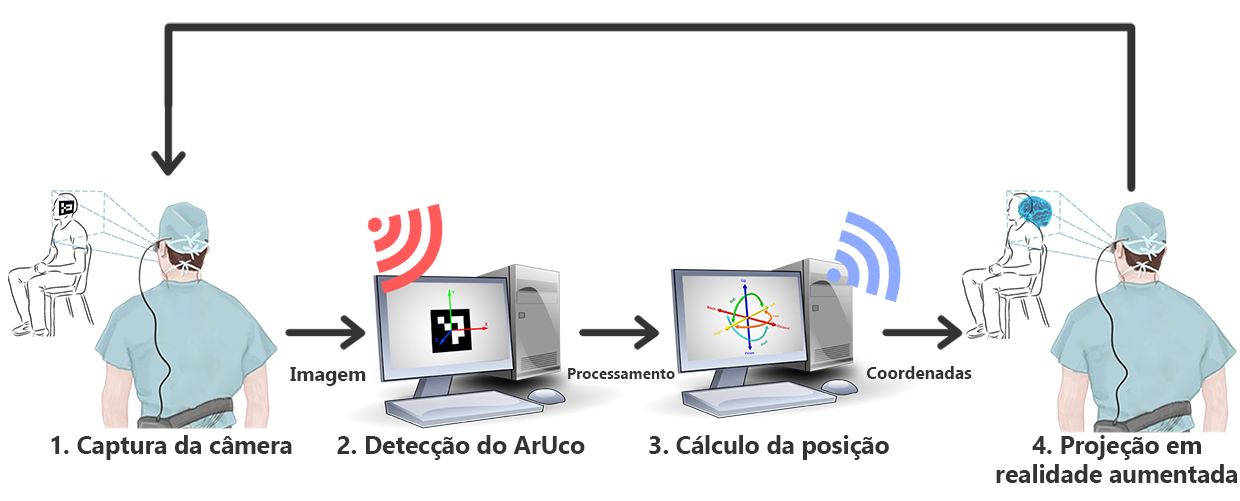
\includegraphics[width=.9\linewidth]{figuras/System schematic.png}
    \caption{A figura representa o funcionamento do sistema. (1) Captura a imagem do paciente e envia para o computador. (2) Faz uma varredura na imagem e identifica o marcador ArUco. (3) Calcula a posição do marcador e envia as coordenadas para os óculos. (4) Recebe as informações e exibe a projeção para o usuário e então retorna para o passo 1. Fonte: Autor.}
    \label{fig:arc}
\end{figure}

\subsection{Comunicação}

A parte prática da programação do sistema teve o desafio de conciliar a comunicação do computador programado em \textit{Python} com os óculos programados em \textit{Unity}. As pesquisas na \textit{web} demonstraram essa comunicação via \textit{TCP/IP} com a utilização de \textit{network sockets} \cite{socket-tutorial}. No entanto, o que precisava ser feito é a transmissão de vídeo em tempo real (\textit{video streaming}), essa ocasião é diferente do envio de uma mensagem de texto, que está na ordem de centenas de \textit{bytes}, uma única imagem pode carregar milhões de \textit{bytes} de informação.

% \begin{figure}[ht]
%     \centering
%     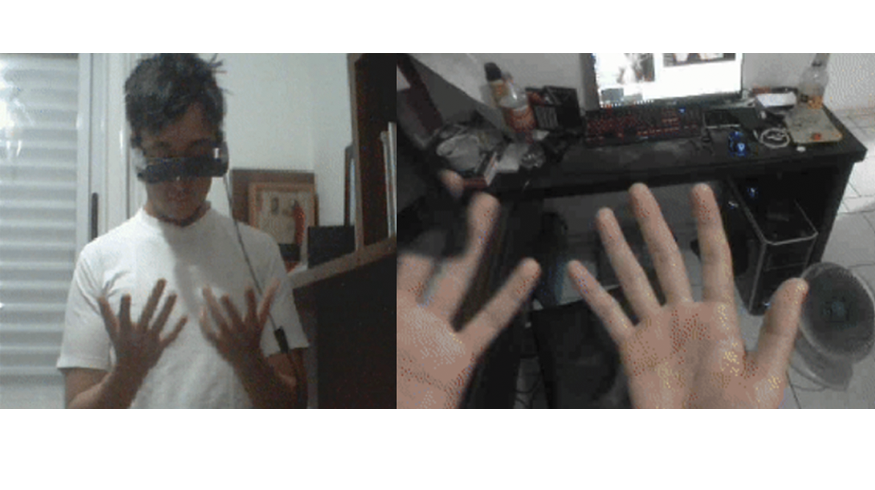
\includegraphics[width=.6\linewidth]{figuras/comm.png}
%     \caption{Êxito da transmissão em tempo real das imagens dos óculos. Fonte: Autor.}
%     \label{fig:communication}
% \end{figure}

Nos testes iniciais, a tentativa foi realizar o processo contínuo de obturação de foto e envio dos dados via \textit{TCP} ao computador. Porém, ocasionalmente, a visualização da imagem era cortada horizontalmente, parecendo que "faltou um pedaço"\(\,\). Isso ocorre pois no processo de recepção de dados do \textit{socket}, a instrução de leitura não sabe o tamanho do arquivo a ser recebido da rede, i.e, o computador não saber o tamanho da imagem eventualmente causava a renderização parcial das informações da foto, resultando em uma imagem defeituosa.

\begin{figure}[ht]
    \centering
        \begin{subfigure}{.45\textwidth}
            \centering
            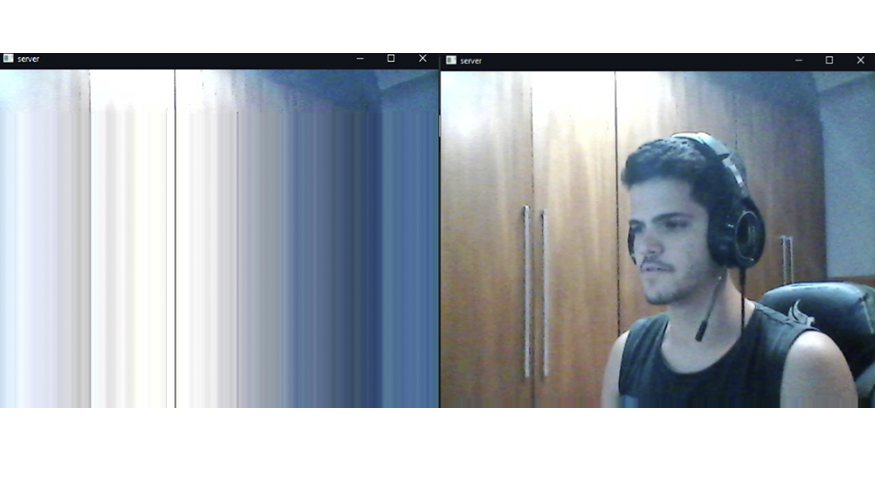
\includegraphics[width=.95\linewidth]{figuras/header.png}
    \caption{Comparação entre uma imagem defeituosa e imagem corrigida com o \textit{header}.}
    \label{fig:header}
        \end{subfigure}
        \begin{subfigure}{.45\textwidth}
            \centering
            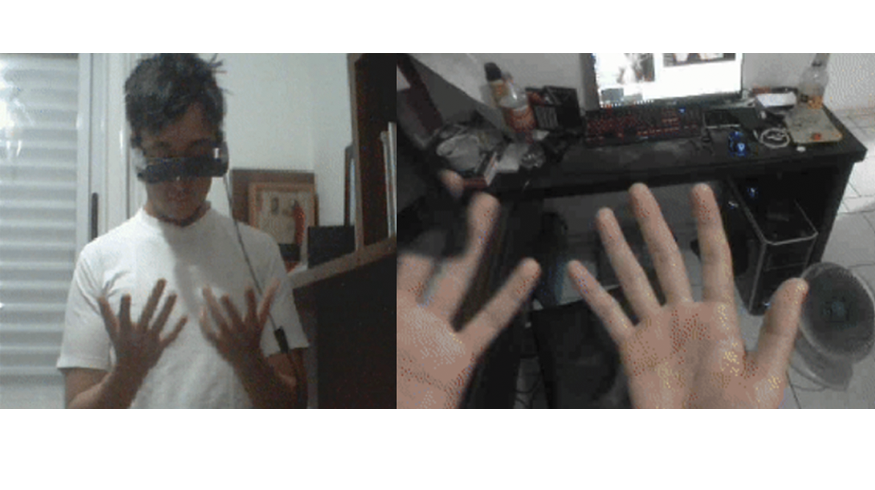
\includegraphics[width=.95\linewidth]{figuras/comm.png}
            \caption{Êxito na transmissão em tempo real das imagens dos óculos para o computador.}
            \label{fig:communication}
        \end{subfigure}
        \caption{Resultados dos testes de comunicação Fonte: Autor.}
        \label{fig:comm-tests}
\end{figure}

% \begin{figure}[ht]
%     \centering
%     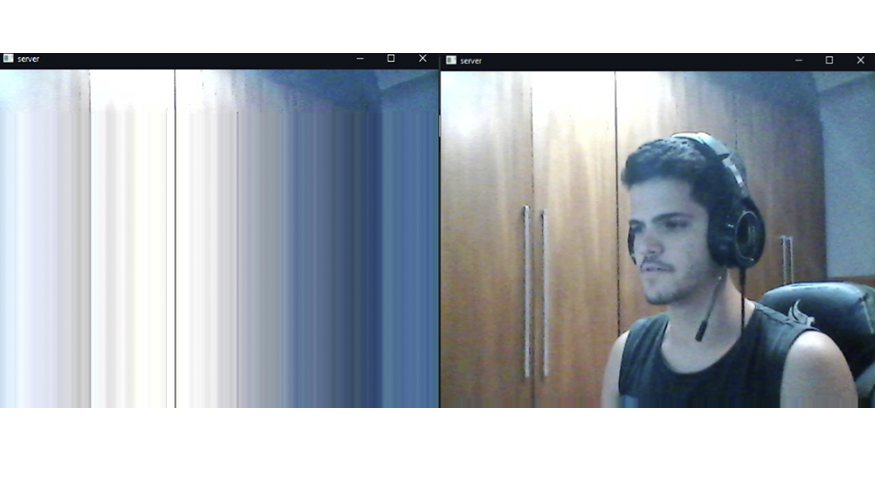
\includegraphics[width=.6\linewidth]{figuras/header.png}
%     \caption{(A) Falha na transmissão\(\,\)(B) Imagem real. Fonte: Autor.}
%     \label{fig:header}
% \end{figure}

% \begin{figure}[ht]
%     \centering
%     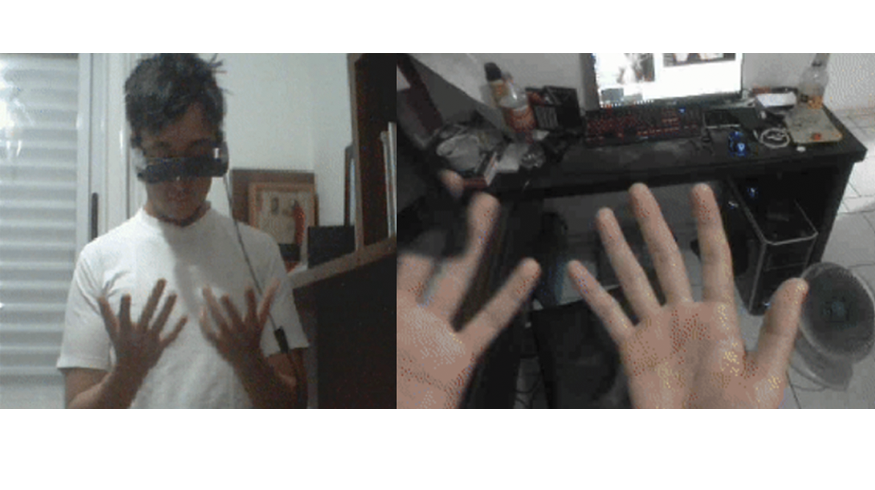
\includegraphics[width=.65\linewidth]{figuras/comm.png}
%     \caption{Transmissão em tempo real das imagens dos óculos. Fonte: Autor.}
%     \label{fig:communication}
% \end{figure}

A solução desse problema foi fazer um envio de uma mensagem de tamanho fixo (\textit{header}) avisando ao computador o tamanho da próxima imagem, garantindo a captura completa da informação de cada foto (Figura \ref{fig:header}). Esse estudo e investigação do problema ampliou muito os conhecimentos de redes e seus protocolos de comunicação. Foi possível adquirir um resultado melhor que o esperado na transmissão de vídeo, obtendo uma taxa superior a 20 quadros por segundo, sua variação é sensível ao conteúdo da imagem por causar variação na taxa de compressão do formato \textit{JPEG} (\textit{Joint Photographic Experts Group}). 

\subsection{Estimação da posição da projeção}

A aplicação objetiva exibir os detalhes da anatomia cerebral de um paciente em AR para auxiliar os procedimentos operatórios de um neurocirurgião. Para isso, devemos utilizar um método que estime a relação entre o mundo real e virtual para sobrepormos a cabeça do paciente com a vista 3D dos seus dados da tomografia computadorizada. A procura desse método é o objeto de pesquisa de muitas referências bibliográficas. Nesse ponto da pesquisa, o projeto pode receber os métodos pesquisados por outros estudantes do laboratório, no entanto, optamos por um método com baixa complexidade para darmos ênfase no objetivo de completarmos todo o sistema e, em um futuro breve, torná-lo em algo mais adequado para o ambiente cirúrgico.

O método de estimação escolhido foi a detecção de marcadores fiduciais nativos da biblioteca do \textit{OpenCV}, o \textit{ArUco}. A estratégia de marcadores, especificamente os com forma quadrada, é comumente utilizada em aplicações de realidade aumentada pela sua rápida responsividade e robustez \cite{Romero-Ramirez2018}. Ele é especial por ter quatro pontos proeminentes (os quatro vértices) que facilitam sua detecção e seu conteúdo interno, preenchido com um padrão único, serve de identificador para o computador \cite{Poroykov2020}.

\begin{figure}[ht]
    \centering
    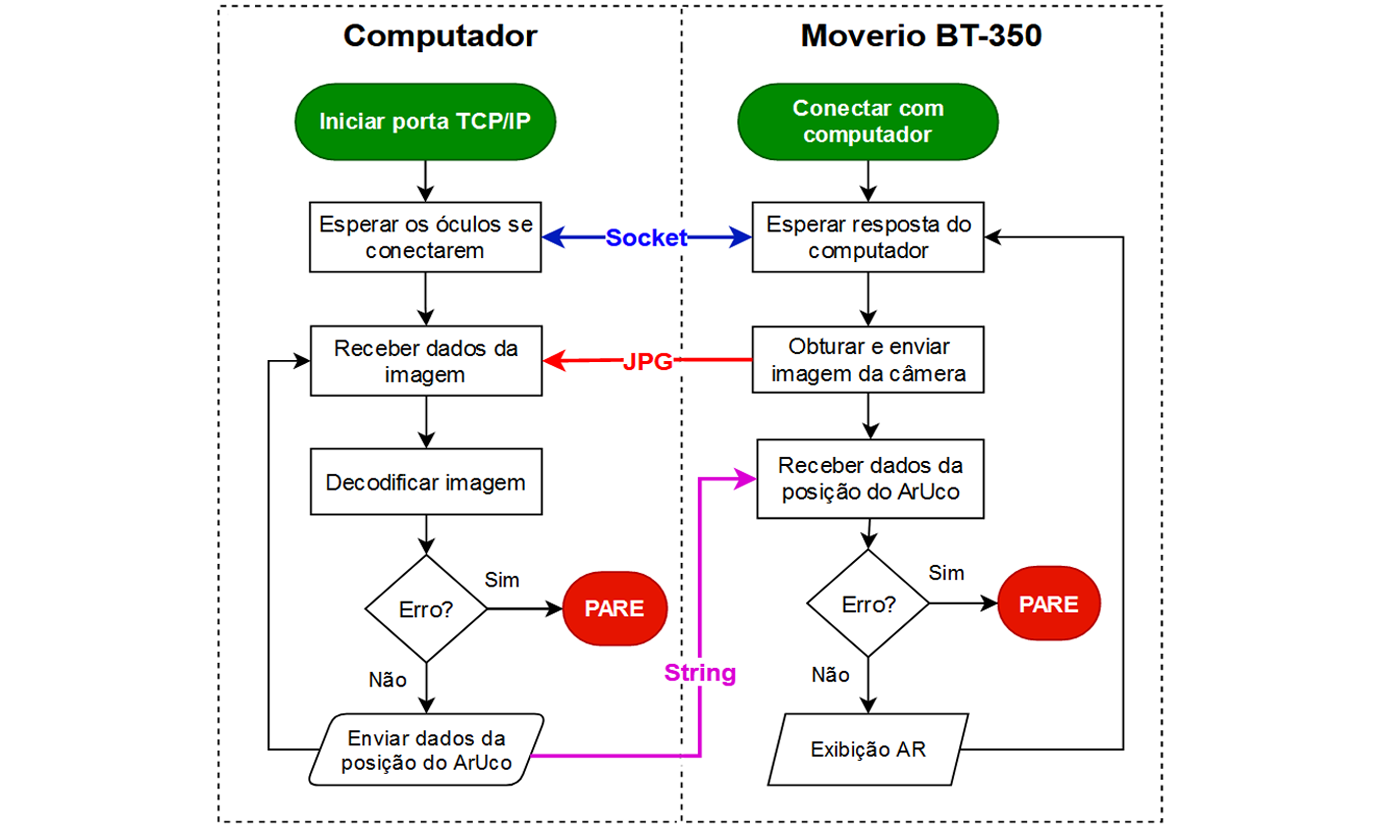
\includegraphics[width=1\linewidth]{figuras/flowchart.png}
    \caption{Fluxograma dos processos da execução do \textit{VCranium}. Fonte: Autor.}
    \label{fig:flowchart}
\end{figure}

\newpage

O algoritmo da detecção \textit{ArUco} foi implementado junto ao programa \textit{Python} do computador. Esse módulo tem como entrada uma imagem dos óculos e saída as coordenadas da posição e rotação do marcador. Os dados são formatados em uma mensagem de tamanho fixo e enviado por \textit{TCP}, semelhante ao \textit{header} da imagem. Na rotina de execução dos óculos, ele primeiro obtura a imagem e envia para o computador, então ele espera a resposta com as informações do \textit{ArUco} correspondentes à imagem e por fim ele posiciona a projeção AR. Na detecção de quaisquer erros de formatação dos \textit{header}, são emitidos como erros fatais no programa, parando todos os processos da execução, vistos no fluxograma da figura \ref{fig:flowchart}.

\subsection{\textit{User Interface}}

Para a criação da interface, demos mais atenção ao funcionamento da projeção das imagens nas lentes dos óculos. A tecnologia empregada é a \textit{Si-OLED (Silicon - Organic Light-Emitting Diode)} que tem a característica de exibir os \textit{pixels} pretos como regiões desligadas de \textit{LED}, i.e, áreas escuras são regiões transparentes e áreas claras são regiões visíveis. Pensando nisso, a interface apresenta as partes interativas mais claras, para chamar atenção do usuário, e um fundo preto para causar um efeito transparente (Figura \ref{fig:ui1}).

% \begin{figure}[ht]
%     \centering
%         \begin{subfigure}{.45\textwidth}
%             \centering
%             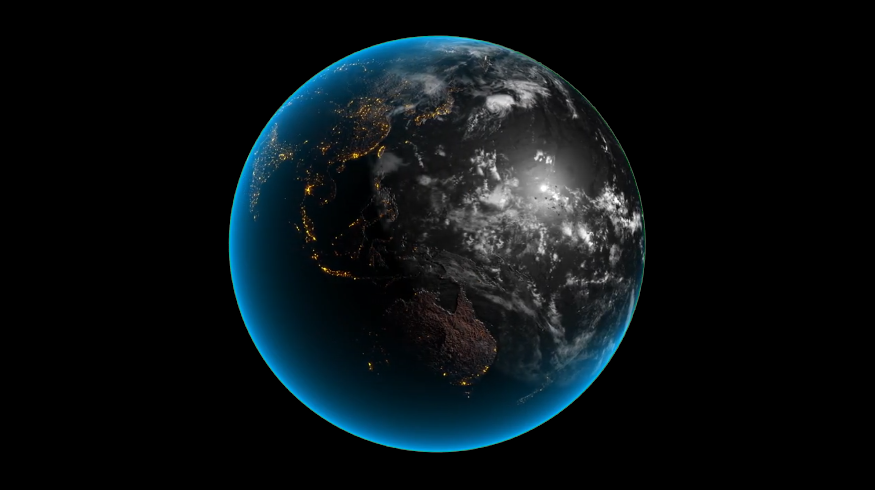
\includegraphics[width=.95\linewidth]{figuras/planeta.png}
%             \caption{Imagem modificada com fundo preto.}
%             \label{fig:planet}
%         \end{subfigure}
%         \begin{subfigure}{.45\textwidth}
%             \centering
%             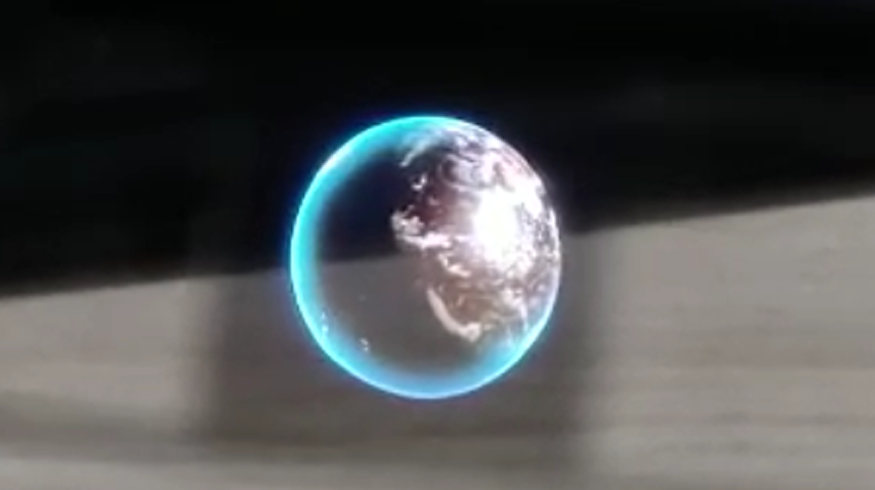
\includegraphics[width=.95\linewidth]{figuras/planetaAR.png}
%             \caption{Exibição transparente nos óculos.}
%             \label{fig:planetAR}
%         \end{subfigure}
%         \caption{As regiões escuras da imagem são vistos como transparência no \textit{display} dos óculos. Ilustração obtida de \cite{planet}. Fonte: Autor.}
%         \label{fig:transparente}
% \end{figure}

\begin{figure}[ht]
    \centering
        \begin{subfigure}{.45\textwidth}
            \centering
            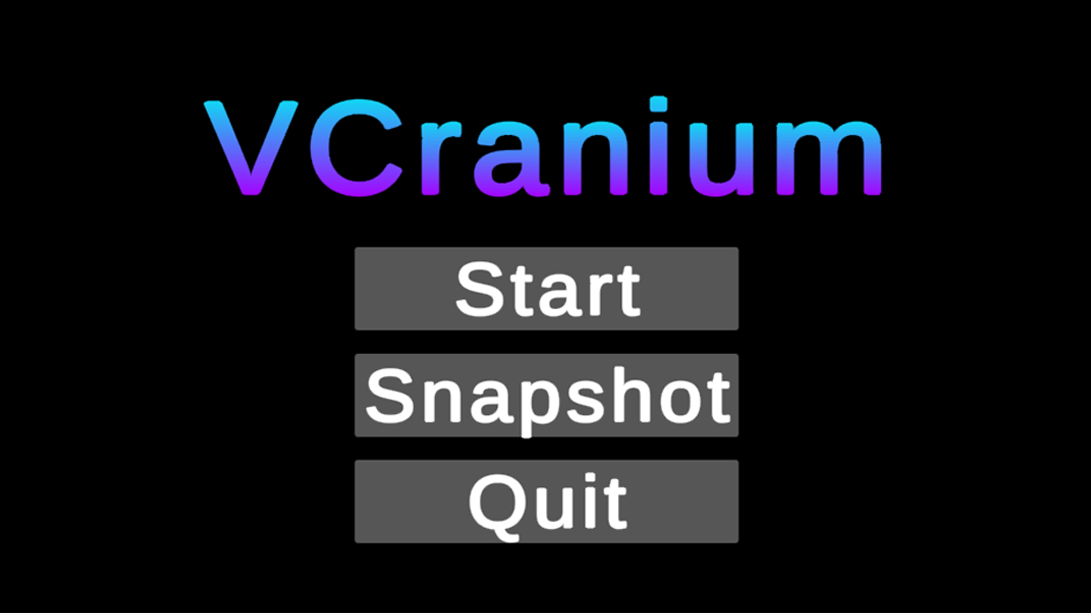
\includegraphics[width=.95\linewidth]{figuras/vcranium_main.png}
            \caption{Menu principal do programa}
            \label{fig:vcranium-connect}
        \end{subfigure}
        \begin{subfigure}{.45\textwidth}
            \centering
            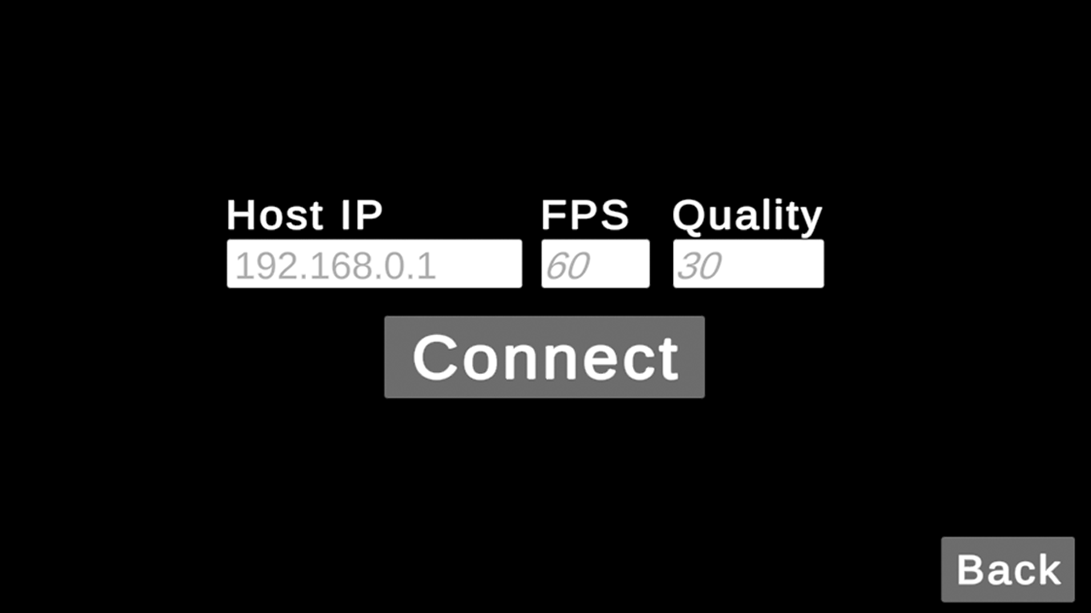
\includegraphics[width=.95\linewidth]{figuras/vcranium_connect.png}
            \caption{Tela de conexão com computador}
            \label{fig:vcranium2-connect}
        \end{subfigure}
        \caption{Imagens da interface do \textit{VCranium}. Fonte: Autor.}
        \label{fig:ui1}
\end{figure}




